%Einfache Vorlage fŸr eine mit Latex realisierte Hausarbeit von http://www.studieren-info.de
%Du kannst diese Vorlage fŸr deine Hausarbeit beliebig anpassen%


%-------------------
%Beginn des Kopfbereiches
%-------------------

%Wir verwenden eine DIN-A4-Seite und die Schriftgrš§e 13.
\documentclass[a4paper,13pt]{scrartcl} 


\usepackage{ucs}
\usepackage[utf8x]{inputenc}


%Diese drei Pakete benštigen wir fŸr die Umlaute, Deutsche Silbentrennung etc.
%Apple-Nutzer sollten anstelle von \usepackage[latin1]{inputenc} das Paket \usepackage[applemac]{inputenc} verwenden
%\usepackage[latin1]{inputenc}
\usepackage[ngerman]{babel}
\usepackage[T1]{fontenc}

%Das Paket erzeugt ein anklickbares Verzeichnis in der PDF-Datei.
\usepackage{hyperref}

%Das Paket wird fŸr die anderthalb-zeiligen Zeilenabstand benštigt
\usepackage{setspace}

%EinrŸckung eines neuen Absatzes
\setlength{\parindent}{0em}

%Definition der RŠnder
\usepackage[paper=a4paper,left=30mm,right=30mm,top=30mm,bottom=30mm]{geometry} 

\usepackage{graphicx}

%Abstand der Fu§noten
\deffootnote{1em}{1em}{\textsuperscript{\thefootnotemark\ }}

%Regeln, bis zu welcher Tiefe (section,subsection,subsubsection) †berschriften angezeigt werden sollen (Anzeige der †berschriften im Verzeichnis / Anzeige der Nummerierung)
\setcounter{tocdepth}{3}
\setcounter{secnumdepth}{3}

%-------------------
%Ende des Kopfbereiches
%-------------------




%-------------------
%Hier beginnt der Text deiner Hausarbeit
%-------------------
\begin{document}


%Beginn der Titelseite
\begin{titlepage}
\begin{small}
\vfill {Universität Hamburg \\ Fachbereich Informatik \\ Proseminar Lokale Rechner- und Mobilnetze \\ Sommersemester 2014 \\ Dr. Klaus-Dieter Heidtmann }
\end{small}


\begin{center}
\begin{Large}
\vfill {\textsf{\textbf{
Architekturen und Standards für Rechnernetze und Mobilnetze: 
Wireless Local Area Network
}}}
\end{Large}
\end{center}


\begin{small}
\vfill Juschua Stock \\ David Kirchhausen Monteiro \\ Frederik Wille \\
\today
\end{small}

\end{titlepage}
%Ende der Titelseite


%Inhaltsverzeichnis (aktualisiert sich erst nach dem zweiten Setzen)
\tableofcontents
\thispagestyle{empty}

%Beginn einer neuen Seite
\clearpage

%Anderthalbzeiliger Zeilenabstand ab hier
\onehalfspacing

\pagestyle{plain}


\section{Einleitung}
\subsection{Was ist WLAN?}
Als WLAN (Wireless Local Area Network) bezeichnet man ein lokales Funknetz, das meist einen Standard der IEEE-802.11 Familie implementiert. In vielen Ländern wird für diese Implementationen auch oft der Begriff "WiFi" verwendet (siehe "WlAN, WiFi - Begriffserklärung" im nächsten Kapitel.\\
WLAN ermöglicht heutzutage einen einfachen Zugang zum Internet und hat in sehr vielen Privat- und Berufsstätten Einzug gefunden. Besonders beliebt sind WLAN-Netze in Eigenheimen, wodurch meist auf der gesamten Wohnfläche ein drahtloser Netzwerkkommunikations- und Internetservice bereitgestellt wird. Außerdem sind die meisten Universitäten, Flughäfen, sowie viele Cafés und Restaurants mit sogenannten Hot-Spots ausgestattet, die je nach Bedarf ihr WLAN-Netz der Öffentlichkeit zugänglich machen können.\\
Seit seiner Entstehung wurde WLAN-Netzen immer mehr Beachtung geschenkt und ihre Bedeutung ist stetig gewachsen. Durch diese enorme Popularität und mittlerweile großen Ausbreitung benutzen die meisten Mitglieder unserer Gesellschaft täglich auf die eine oder andere Art WLAN-Netze, sei es mit Mobilgeräten ("Smartphones", Tablets, mobilen Computern) oder mit Tower-Rechnern.
\subsection{Anforderungen}
Typische Anforderungen an WLANs sind beispielsweise ein möglichst hoher Durchsatz an Daten, eine große Anzahl von Klienten (Mobilstationen) und die Interkonnektion mit leitungsgebundenen Netzen. Letztere ermöglicht beispielsweise die beliebte Anbindung an das weltweite Internet. Außerdem sollen die elektromagnetischen Wellen der WLAN-Netze in einem möglichst großen Bereich empfangen werden können und die Mitgliedschaft in einem WLAN-Netz sollte für einen Klienten möglichst stromsparsam möglich sein (um bspw. Handyakkus zu schonen). Des Weiteren sollte der Betrieb möglichst lizenzfrei möglich sein, um insbesondere Privatpersonen das Einrichten eines WLAN-Netzes nicht zu erschweren. Zu guter Letzt sollte garantiert sein, dass das Konfigurieren neu zu integrierender bzw. auszugliedernder Mobilstationen dynamisch passiert und keinen großen Aufwand seitens des Netzbereitstellers fordert.
\subsection{WLAN, WiFi - Begriffserklärung}
Zwischen den Begriffen WLAN und WiFi steckt ein großer Bedeutungsunterschied, der z.B. in Großbrittanien, Kanada und Spanien kaum beachtet wird. WLAN bezeichnet das Netzwerk selber ("Network"), hinter dem Begriff WiFi steckt die WiFi-Alliance. 1999 gegründet, stellt sie seitdem Interoperabilität zwischen Geräten sicher, indem sie Geräte zertifiziert.\\ Konkret funktioniert das folgendermaßen: Hersteller, die sich nach dem Zertifikat für ihr Produkt sehnen, schicken es der Allianz, die das Produkt umfangreich testet. Insbesondere wird (gegen eine Gebühr) getestet, ob es dem entsprechenden IEEE-Standard entspricht und Interoperabilität ermöglicht. Verläuft die Prüfung erfolgreich, darf der Hersteller das Produkt mit dem bekannten WiFi-Logo kennzeichnen.\\
Hintergrund dieser Zertifizierung ist ein, insbesondere in den 90er-Jahren aufkommender Boom der Technologie, der viele Standardaufweichungen, z.B. durch proprietäre Hardware, mit sich zog und Inkompatibilitätsprobleme mit sich zog.
\subsection{Geschichtlicher Hintergrund, ALOHAnet}
Mit zunehmender Bedeutung und Verbreitung von Computern wurden in der zweiten Hälfte des 20. Jahrhunderts Vernetzungsmöglichkeiten zunehmend wichtiger. Auf der Suche nach neuen, insbesondere drahtlosen Mitteln des Informationsaustausches wurde 1970 an der Universität von Hawaii unter der Leitung von Norman Abramson das sogenannte ALOHAnet entwickelt. Es diente ausschließlich Forschungszwecken. Es war das erste Netz, in dem Nutzer über Funkstrecken auf einen Zentralrechner zugreifen konnten.\\
Konkret verband es den Zentralrechner auf der Insel Oahu mit sieben Standorten auf vier Inseln (siehe Abb.1). Später wurde es, mithilfe des Einsatzes von Repeatern, auf weitere Inseln Hawaiis ausgedehnt. Anfänglich konnten Endgeräte nur auf den Großrechner zugreifen, später war es sogar möglich, mit anderen Endgeräten zu kommunizieren.\\
Technisch war ALOHAnet so aufgebaut, dass ein Broadcast- und ein Random-Access-Kanal paralell genutzt wurden. Die Stationen schickten ihre Datenpakete über den Random-Access-Kanal zum Zentralrechner und erhielten nach erfolgreicher Übertragung eine Nachricht des Empfängers über den Broadcast-Kanal. Bei eventueller gleichzeitiger Übertragung von zwei Nachrichten (bzw. Stationen) schlugen beide Versuche fehl und das Senden wurde nach einer zufällig gewählten Zeitspanne wiederholt. Auf diese Weise wurden die Chancen, dass beide Sender beim nächsten Übertragungsversuch wieder eine Kollision erzeugen, minimiert.

%Abbildung 1: Bild mit Inseln und Rechnern
\begin{figure}[ht]
		\centering
	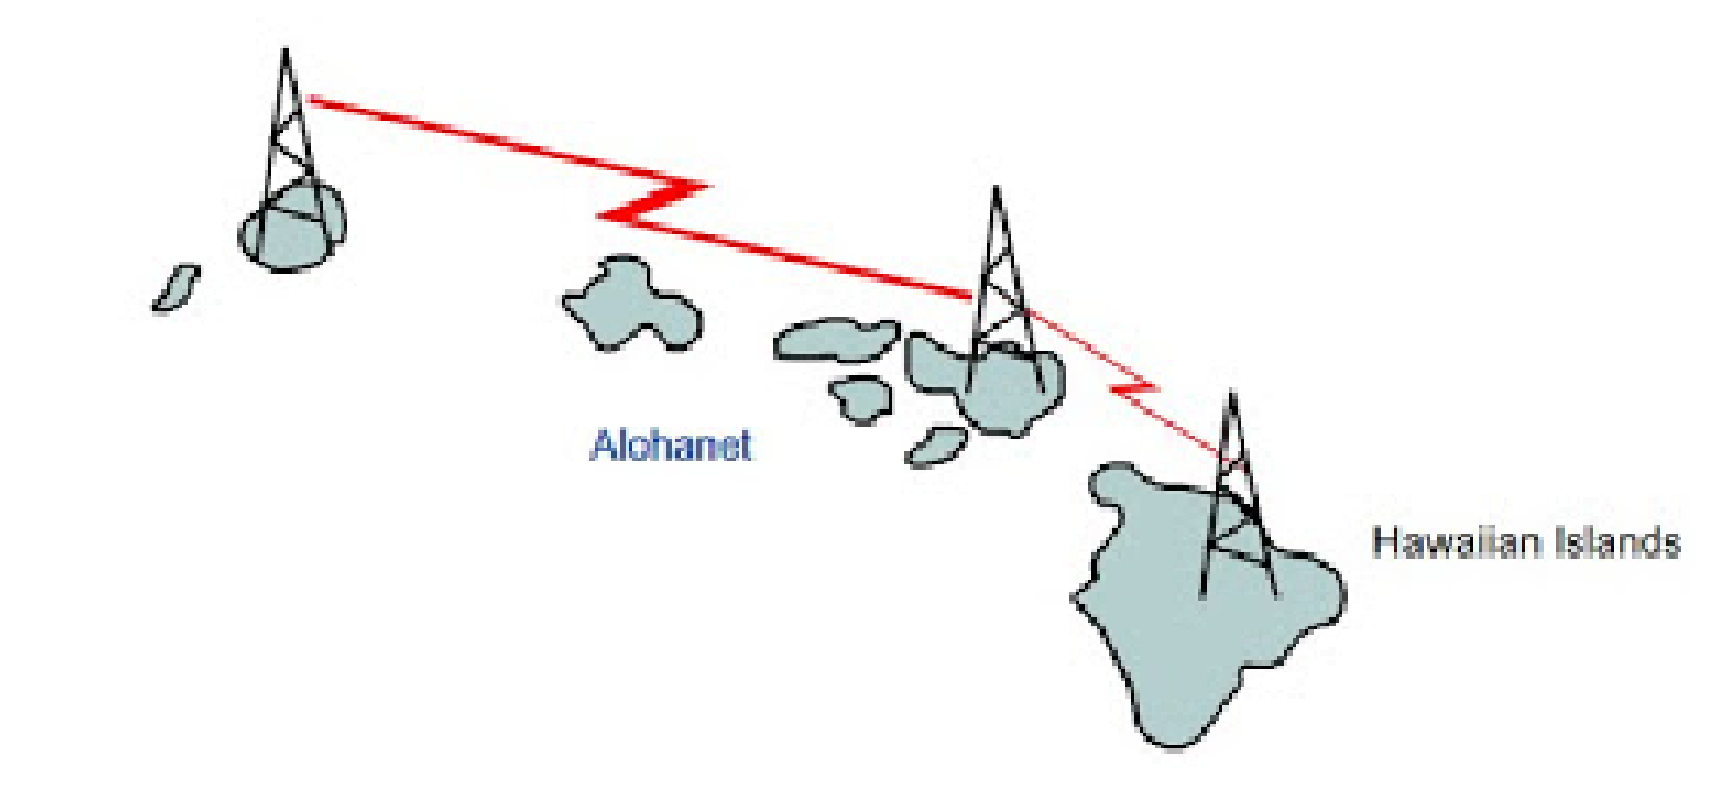
\includegraphics[width=0.5\textwidth]{alohanet.eps}
		\caption{Schematische Darstellung des ALOHAnet}
		\label{fig1}
\end{figure}

\section{Functionalität}

\subsection{Infrastruktur}

shit

\subsection{Ad-Hoc}

noch mehr shit

\section{technische Aspekte}
\subsection{IEEE}
Das Institute of Electrical and Electronics Engineers\footnote{Der volle Name wurde inzwischen fast komplett aufgegeben und wird nur noch für offizielle Dokumente genutzt} ist ein im Jahre 1963 gegründerter Berufsverband von Elektro- und Informationstechnik Ingenieuren. Neben den weitverbreiteten Standards veröffentlicht das IEEE einige sehr angesehene Fachzeitschriften und hält Tagungen. 
Untergliedert ist die IEEE in 
\subsubsection{Unterüberschrift}
foobar
\subsubsection{Unterüberschrift}
asfs
\section{Sicherheit}
\subsection{RC4}
\subsection{WEP}
\subsection{WPA}
\subsection{WPA2}
\subsection{Gesundheitsaspekte}


\section{Schluss}
afgdfv

%Beginn einer neuen Seite
\clearpage

\section{Literaturverzeichnis}

Musterfrau, Renate: Muster. Frankfurt 2003.


Mustermann, Helmut: Noch ein Muster. Mit einer Einleitung hrsg. von Frank Muster. Frankfurt 2003.

ALOHAnet: http://www.netplanet.org/geschichte/arpa.shtml
http://de.wikipedia.org/wiki/ALOHAnet
Abbildung: Quelle: http://dixland.blogspot.de/2010/09/first-lan-in-world-was-original-version.html

\end{document}
%-------------------
%Hier endet der Text deiner Hausarbeit
%-------------------